\documentclass[11pt]{article}
\usepackage[utf8]{inputenc}
\usepackage{amsmath}
\usepackage{amssymb}
\usepackage{graphicx}
\usepackage{hyperref}
\usepackage[parfill]{parskip}
\let\oldemptyset\emptyset
\let\emptyset\varnothing


\title{\textbf{Esssentials of Applied Data Analysis\\
				IPSA-USP Summer School 2017}\newline\\
				The Basics of Set Theory}

\author{Leonardo Sangali Barone\\ \href{leonardo.barone@usp.br}{leonardo.barone@usp.br}}
\date{jan/17}

\begin{document}

\maketitle

\section*{Set Theory}

Basic notions and notation of set theory.

\subsection*{First concepts and notation}

	\begin{itemize}
		\item Sets are a list or collection of objects.
		\item These objects are elements.
		\item $\emptyset$ is the empty set.
		\item $p \in A$: is p is an element in the set $A$.
		\item $A \subset B$: $A$ is a subset of $B$ 
	\end{itemize}


\subsection*{Set Theory - operations}

	\begin{itemize}
		\item $A \cup B$: union of $A$ and $B$.
		\begin{itemize}
			\item $p \in (A \cup B$): p is an element of $A$ \textbf{OR} $B$.
		\end{itemize}
		\item $A \cap B$: intersection of $A$ an $B$.
		\begin{itemize}
			\item $p \in (A \cup B$): p is an element of $A$ \textbf{AND} $B$.
		\end{itemize}
		\item If $A \cap B$ is equal to $\emptyset$, then A and B are \textbf{disjoint} sets.
		\item $A^c$ ($A'$, \textasciitilde$A$ or simply \emph{not A}) is the set of all elements that does not belong to $A$. $A^c$ is the complement of $A$. 

	\end{itemize}

\subsection*{Venn Diagrams}
 We can represent sets with diagrams. These are called ``Venn Diagrams''. See Figure~\ref{f1} and locate the following sets as a quick exercise:\\

\begin{tabular}{llll}
	1) $A \cup B$ & 5) $(A \cup B) \cup C$ & 9) $A^c$ & 13) $((A \cap B) \cap C)^c$\\
	2) $A \cap B$ & 6) $(A \cap B) \cap C$ & 10) $(A \cap B)^c$ & 14) $((A \cup B) \cap C)^c$\\
	3) $A \cup C$ & 7) $(A \cup B) \cap C$ & 11) $(A \cup C)^c$ &\\
	4) $A \cap C$ & 8) $(A \cap B) \cup C$ & 12) $((A \cup B) \cup C)^c$ &\\
\end{tabular}

\begin{figure}[htp]
\centering
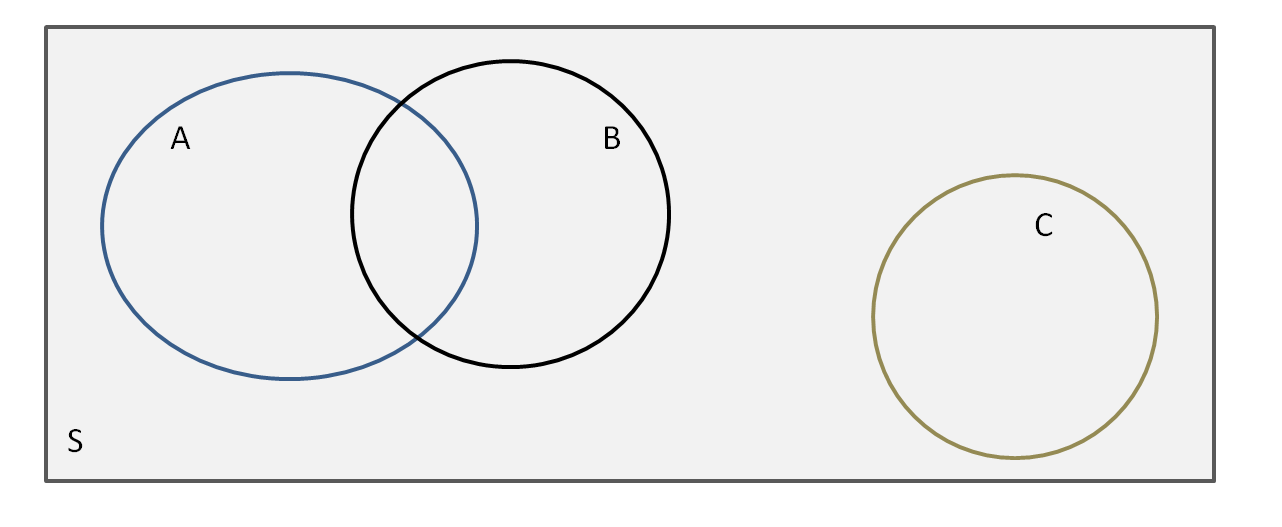
\includegraphics[scale=0.40]{venn.png}
\caption{Venn Diagrams}
\label{f1}
\end{figure}

\end{document}